\renewcommand{\thepage}{\CoverName}
\begin{titlepage}
	\begin{tikzpicture}[remember picture,overlay]
		\node [align=center] at (current page.north)
		{\begin{tikzpicture}[remember picture, overlay]
			\fill[fill=Periwinkle ] (-9,0) rectangle (9,-0.5);
			\node[anchor=north] at (0,-0.5) {\garamond\quitelarge\textit{Почти наверное достаточное}\\
				\garamond\quitelarge\textit{учебное пособие}};
			\fill[fill=Periwinkle] (-9,-4) rectangle (9,-10);
			\node[anchor=west,align=left] at (-8.5,-7) {\garamond\veryhuge\color{white}Теория вероятностей\\
				\garamond\veryhuge\color{white}и математическая\phantom{Мр} \\
				\garamond\veryhuge\color{white}статистика\phantom{М}};
			\node[inner sep=0pt] (whitehead) at (0,-18)
			{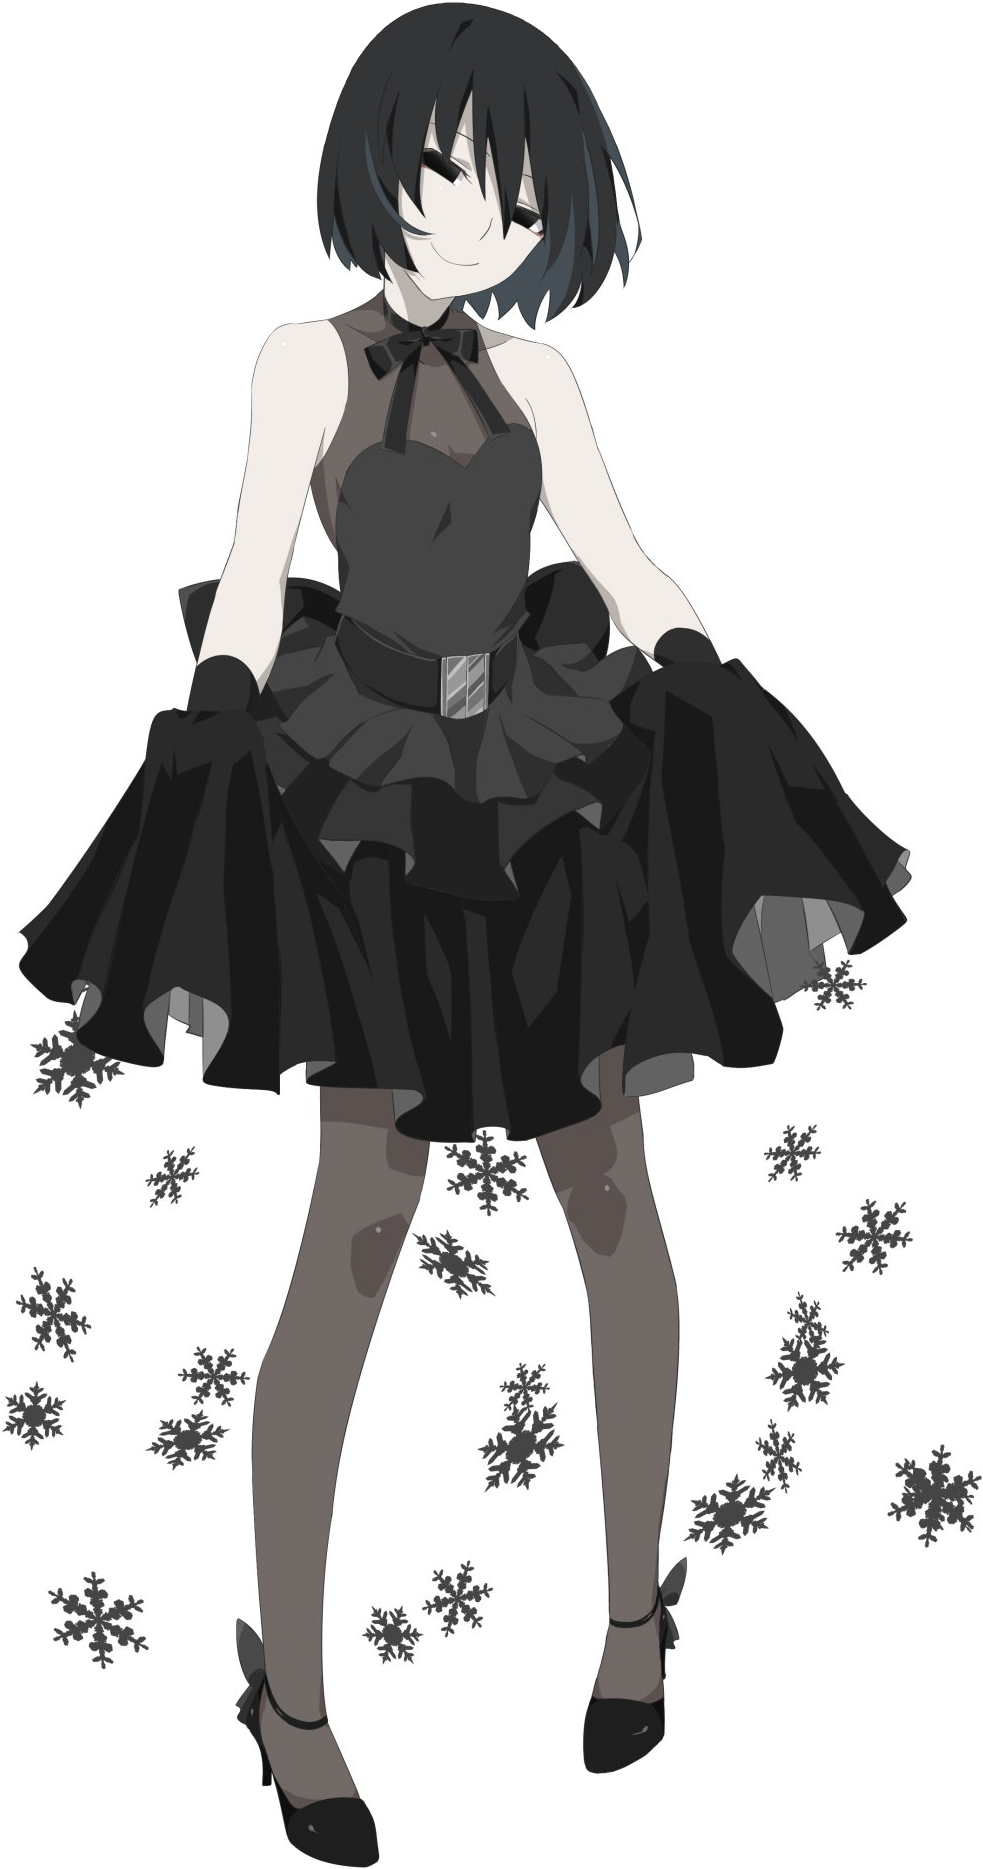
\includegraphics[width=.542\textwidth]{src/new_ougi_2.png}};
			\end{tikzpicture}};
		\node [shift={(-5cm,-5cm)}] at (current page.north east)
		{\begin{tikzpicture}[remember picture, overlay]
			\draw[fill=black] (0,5) -- (1.5,5) -- (5,1.5) -- (5,0) -- cycle ;
			\node[inner sep=0pt,rotate=-45] (rev) at (2.9,2.9) {\garamond\verylarge\color{white}\textbf{2.5-е издание}};
			\end{tikzpicture}};
		\node [align=center] at (current page.south)
		{\begin{tikzpicture}[remember picture, overlay]
			\node[anchor=south west, align=left] at (-9,2) {\gillius\verylarge\textbf{CMC MSU}};
			\node[anchor=south east, align=right] at (9,2) {\garamond\quitelarge\textit{@MandaloreUltimate}};
			\end{tikzpicture}};
	\end{tikzpicture}
\end{titlepage}